% % % % % % % % % % % % % % % % % % % % % % % % % % % % % % % % % %
\documentclass[runningheads]{llncs}

% packages
\usepackage{xspace}
\usepackage{ifthen}
\usepackage{amsbsy}
\usepackage{amssymb}
\usepackage{balance}
\usepackage{booktabs}
\usepackage{graphicx}
\usepackage{multirow}
\usepackage{needspace}
\usepackage{microtype}
\usepackage{bold-extra}

% constants
\newcommand{\Title}{Aspect-based refactoring}
\newcommand{\TitleShort}{\Title}
\newcommand{\Authors}{Santiago Vidal, Claudia Marcos, Alexandre Bergel, Gabriela Ar\'evalo}
\newcommand{\AuthorsShort}{S. Vidal, C. Marcos, A. Bergel, G. Ar\'evalo}

% references
\usepackage[colorlinks]{hyperref}
\usepackage[all]{hypcap}
\setcounter{tocdepth}{2}
\hypersetup{
	colorlinks=true,
	urlcolor=black,
	linkcolor=black,
	citecolor=black,
	plainpages=false,
	bookmarksopen=true,
	pdfauthor={\Authors},
	pdftitle={\Title}}

\def\chapterautorefname{Chapter}
\def\appendixautorefname{Appendix}
\def\sectionautorefname{Section}
\def\subsectionautorefname{Section}
\def\figureautorefname{Figure}
\def\tableautorefname{Table}
\def\listingautorefname{Listing}

% source code
\usepackage{xcolor}
\usepackage{textcomp}
\usepackage{listings}
\definecolor{source}{gray}{0.9}
\lstset{
	language={},
	% characters
	tabsize=3,
	upquote=true,
	escapechar={!},
	keepspaces=true,
	breaklines=true,
	alsoletter={\#:},
	breakautoindent=true,
	columns=fullflexible,
	showstringspaces=false,
	basicstyle=\footnotesize\ttfamily,
	% background
	frame=single,
    framerule=0pt,
	backgroundcolor=\color{source},
	% numbering
	numbersep=5pt,
	numberstyle=\tiny,
	numberfirstline=true,
	% captioning
	captionpos=b,
	% formatting (html)
	moredelim=[is][\textbf]{<b>}{</b>},
	moredelim=[is][\textit]{<i>}{</i>},
	moredelim=[is][\color{red}\uwave]{<u>}{</u>},
	moredelim=[is][\color{red}\sout]{<del>}{</del>},
	moredelim=[is][\color{blue}\underline]{<ins>}{</ins>}}
\newcommand{\ct}{\lstinline[backgroundcolor=\color{white},basicstyle=\footnotesize\ttfamily]}
\newcommand{\lct}[1]{{\small\tt #1}}

% tikz
% \usepackage{tikz}
% \usetikzlibrary{matrix}
% \usetikzlibrary{arrows}
% \usetikzlibrary{external}
% \usetikzlibrary{positioning}
% \usetikzlibrary{shapes.multipart}
% 
% \tikzset{
% 	every picture/.style={semithick},
% 	every text node part/.style={align=center}}
% \tikzexternalize[prefix=figures/]{quality}

% proof-reading
\usepackage{xcolor}
\usepackage[normalem]{ulem}
\newcommand{\ra}{$\rightarrow$}
\newcommand{\ugh}[1]{\textcolor{red}{\uwave{#1}}} % please rephrase
\newcommand{\ins}[1]{\textcolor{blue}{\uline{#1}}} % please insert
\newcommand{\del}[1]{\textcolor{red}{\sout{#1}}} % please delete
\newcommand{\chg}[2]{\textcolor{red}{\sout{#1}}{\ra}\textcolor{blue}{\uline{#2}}} % please change
\newcommand{\chk}[1]{\textcolor{ForestGreen}{#1}} % changed, please check

% comments \nb{label}{color}{text}
\newboolean{showcomments}
\setboolean{showcomments}{true}
\ifthenelse{\boolean{showcomments}}
	{\newcommand{\nb}[3]{
		{\colorbox{#2}{\bfseries\sffamily\scriptsize\textcolor{white}{#1}}}
		{\textcolor{#2}{\sf\small$\blacktriangleright$\textit{#3}$\blacktriangleleft$}}}
	 \newcommand{\version}{\emph{\scriptsize$-$Id$-$}}}
	{\newcommand{\nb}[2]{}
	 \newcommand{\version}{}}
\newcommand{\rev}[2]{\nb{Reviewer #1}{red}{#2}}
\newcommand{\ab}[1]{\nb{Alexandre}{blue}{#1}}
\newcommand{\lr}[1]{\nb{Lukas}{orange}{#1}}

% graphics: \fig{position}{percentage-width}{filename}{caption}
\DeclareGraphicsExtensions{.png,.jpg,.pdf,.eps,.gif}
\graphicspath{{figures/}}
\newcommand{\fig}[4]{
	\begin{figure}[#1]
		\centering
		\includegraphics[width=#2\textwidth]{#3}
		\caption{\label{fig:#3}#4}
	\end{figure}}

% abbreviations
\newcommand{\ie}{\emph{i.e.,}\xspace}
\newcommand{\eg}{\emph{e.g.,}\xspace}
\newcommand{\etc}{\emph{etc.}\xspace}
\newcommand{\etal}{\emph{et al.}\xspace}

% lists
\newenvironment{bullets}[0]
	{\begin{itemize}}
	{\end{itemize}}

\newcommand{\seclabel}[1]{\label{sec:#1}}

% D O C U M E N T
% % % % % % % % % % % % % % % % % % % % % % % % % % % % % % % % % %
\begin{document}

% T I T L E
% % % % % % % % % % % % % % % % % % % % % % % % % % % % % % % % % %

\title{\Title}
\titlerunning{\TitleShort}

\author{\Authors} 
\authorrunning{\AuthorsShort}

\institute{ISISTAN Research Institute, Faculty of Sciences,\\
UNICEN University, Campus Universitario, Tandil, Buenos Aires, Argentina\\
PLEIAD Lab, Department of Computer Science (DCC),\\
	University of Chile, Santiago, Chile,
...}

\maketitle

% A B S T R A C T
% % % % % % % % % % % % % % % % % % % % % % % % % % % % % % % % % %

\begin{abstract}
an abstract
\end{abstract}

% % % % % % % % % % % % % % % % % % % % % % % % % % % % % % % % % %
\section{Introduction}\seclabel{introduction}

The story to tell in this paper is the following one:
1) We have the actual Mondrian code
2) Santiago have extracted the CC into pragmas
3) He has identified different possible pragmas. Here some patterns could be identified based on the code (That's the POINT of the paper)
4) Once we have the pragmas, we can think of an injection machine to produce new code.
This new code is semantically equivalent to the original one, but not syntactically the same. This is not so important since all the large set of Mondrian unit tests has the last word on it.

Then the core of the paper will be the Different patterns of hand written code that are rewritten (refactored?) with pragmas 

justificar el xq se quiere refactorizar los cache 

% % % % % % % % % % % % % % % % % % % % % % % % % % % % % % % % % %
\section{Refactoring}\seclabel{refactoring}

The goal of the refactorization was the separation of the \emph{Cache
Concern} from the main class of \emph{Mondrian}: \emph{MOGraphElement}
and its subclasses (\emph{MOEdge}, \emph{MONode}, and \emph{MORoot}).
The refactoring process began with the identification of the caches
and the places where they were used. Six different caches were found:
\emph{cacheShapeBounds}, \emph{cacheForm}, \emph{boundsCache}, \emph{absoluteBoundsCache},
\emph{elementsToDisplayCache}, and \emph{lookupNodeCache}. Each of
them has a different internal structure according on what is stored.
After this initial identification, the fragment of codes in which
the caches were used were grouped together based on the purpose of
its use. The main general purposes identified were:
\begin{itemize}
\item Initialize or reset the cache.
\item Get the data stored in the cache.
\item Store data in the cache.
\end{itemize}
The task of group was achieved with the goal of identifying possible
strategies for refactoring. In this line, some subgroups were found.
These subgroups allowed the identification of code patterns that were
repeated in the use of the caches. Once the patterns were identified,
a refactoring strategy was applied. These steps are described in the
following subsections.


\subsection{Pattern Description\label{sub:Pattern-Identification}}

In this section, the main code pattern are presented. For each pattern
is mentioned its name with a brief description of the pattern and
typical situations in which it appears. Also it is introduced the
number of occurrences of the pattern and a code example. The purpose
of the code examples is to illustrate the occurrences of each pattern
in the proper context. 

Following, the patterns are presented ordered by the number of occurrences.

\emph{Reset Cache}: this pattern represents a situation in which a
cache is resetted. The reset structure is \emph{cache:=resetValue}
where \emph{resetValue} depends on the cache internal structure. Typically,
the \emph{resetValue} is nil or a new of a kind of Dictionary object.
Fourteen occurrences of this pattern were found in the Mondrian code.
Next, the method \emph{resetCache} is presented as an example. In
this method the \emph{Reset Cache} pattern is repeated in four occasions
to reset the caches \emph{boundsCache}, \emph{absoluteBoundsCache},
\emph{cacheShapeBounds}, and \emph{elementsToDisplayCache}.

\begin{lstlisting} 
MOGraphElement>>resetCache 
	self resetElementsToLookup.
	boundsCache := nil. 
	absoluteBoundsCache := nil. 
	cacheShapeBounds := SmallDictionary new. 
	elementsToDisplayCache := nil. 
	self resetMetricCaches
\end{lstlisting}

\emph{Return Cache with Precondition Checking}: this pattern shows
the situation in which a verification is accomplished before access
to a cache with the goal of avoid possible exceptions when the cache
is nil. Typically, the structure of this pattern is: \emph{if (cache==nil)
cache:=newValue. return cache}. Four occurrences of this pattern were
found in the Mondrian code. Next, the method \emph{bounds} is presented
as an example in which boundsCache is accessed.

\begin{lstlisting}
MOEdge>>bounds
	^ boundsCache ifNil: [ boundsCache := self shape computeBoundsFor: self ].
\end{lstlisting}

\emph{Cache Initialization}: this pattern represents a situation in
which a value is assigned to a cache. The structure of the pattern
is only an assignation: cache:=\emph{aValue}. This pattern was found
in two occasions. Next, the method \emph{cacheCanvas} is presented
as an example in which a value is assigned to cacheForm.

\begin{lstlisting}
 MOGraphElement>>cacheCanvas: aCanvas 
	cacheForm := aCanvas form copy: ((self bounds origin + aCanvas origin 
	- (1@1)) extent: (self bounds extent + (2@2))). 
\end{lstlisting}

\emph{Return Cache}: this pattern shows the situation in which a cache
is accessed. The structure of the pattern is the return of the cache:
\emph{return cache}. This pattern was found in two occasions. Next,
the method \emph{shapeBounds} is presented as an example in which
cacheShapeBounds is accessed.

\begin{lstlisting} 
MOGraphElement>>shapeBounds 
	^ cacheShapeBounds 
\end{lstlisting}

Fig. \ref{fig:Pattern-locations-in} shows in which methods the
patterns were found.%
\begin{figure}
\begin{centering}
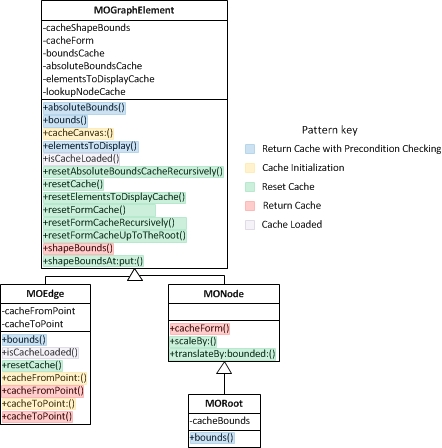
\includegraphics[scale=0.9]{PatternLocation}
\par\end{centering}

\caption{Pattern locations in MOGraphElement hierarchy.\label{fig:Pattern-locations-in}}



\end{figure}

\subsection{Refactoring Strategy}

Once the code patterns were identified, strategies to refactor them
were established. The main constraint to refactoring the code was
the preservation of a good performance of the cache mechanism. 

Several alternatives were explored to encapsulated the \emph{Cache
Concern}. For example, one of the explored mechanisms was the separation
of the concern by means of the definition of an exclusive class for
managing caches. While this solution provided a good modular design,
it introduced indirections to access to the caches. Indirections caused
a poor performance that slows down response times of the cache mechanism.
For this reason, this is not a feasible solution.

After exploring a variety of options such as the use of proxies to
intercept messages, an approach based on code injection was chosen.
This solution has the advantage of encapsulating the concern in a
new unit while the code that it is finally executed after the injection
is similar to the original code of \emph{Mondrian}. So, the performance
is not affected. In order to encapsulate the source code related with
the code patterns the \emph{pragma} mechanism is used. \emph{Pragmas}
are the method annotation syntax implemented by Pharo \cite{PharoByExample}.

The refactoring strategy used was: for each method that contained
code related to the \emph{Cache Concern}, the code related to the
concern was extracted using a pragma that was defined in the method.
The decision of define the pragma inside the method was in order to
allow a better visibility of the code that is injected. The pragmas
used have the structure \emph{<cache: before: '' after: ''>} where
\emph{cache} indicates the name of the cache that will be injected.
The clauses before and after indicate the source code that will be
injected and when it will be injected in regard to the execution of
the method. For example, the pragma \emph{<cache: \#boundsCache before:
'boundsCache := nil' after:''>} indicates that \emph{boundsCache}
will be resetted before the execution of the method in which the pragma
is defined. 

Once that the cache code is extrated into the pragmas, this code is
injected before the execution of the system. Specifically, the automatic
injection of a pragma in a method is achieved following the next steps:
\begin{itemize}
\item A new method is created with the same name that the method that contains
the pragma but with the prefix {}``compute''. For example, if the
name of the method is absoluteBounds, a new method called computeabsoluteBounds
will be created.
\item The code of the original method is copied into the new method.
\item The code inside the original method is replaced by the code pointed
out in the before clause of the pragma.
\item A call to the new method is added at the end of the original method.
\item The code of the after clause of the pragma is added at the end of
the original method.
\end{itemize}
In this way, the injected code is executed after and before of the
execution of the method that contains the pragma. The whole injection
mechanism is summarized in Fig. \ref{fig:Injection-mechanism.}. %
\begin{figure}
\begin{centering}
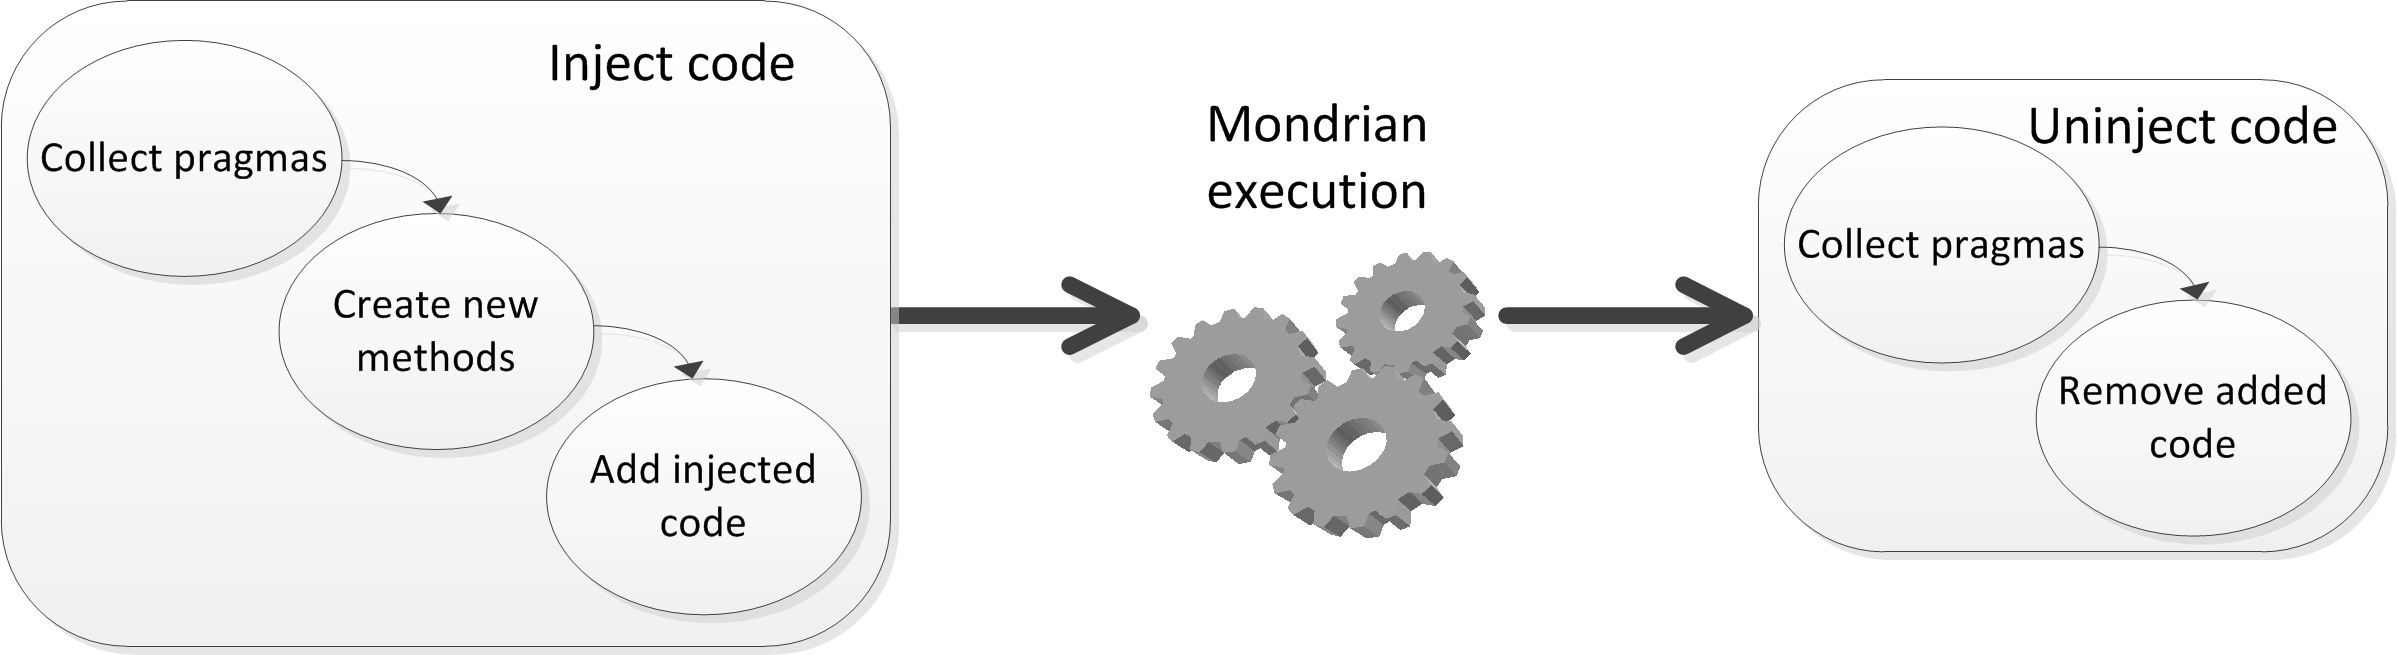
\includegraphics[scale=0.8]{InjectionMechanism}
\par\end{centering}

\caption{Injection mechanism.\label{fig:Injection-mechanism.}}



\end{figure}


Next, the refactorizations applied for each code pattern are presented.

\emph{Reset Cache}: In order to refactor this pattern each statement
that resets a cache was extrated using a pragma. The pragma contains
the code that resets the cache and follows the pattern \emph{cache:=resetValue}.
In regard to when the code is inyected, it depends on the method that
is being restructured. For example, in the case presented in Section
\ref{sub:Pattern-Identification} of the method \emph{resetCache},
a pragma was defined for each reset of a cache leaving a cleaner code
in the method. In this case all the resets are done before the method
call. Even though the order of calls is changed, the method behaviour
is not modified. Following, the refactored code is presented:

\begin{lstlisting} 
MOGraphElement>>resetCache 
	<cache: #absoluteBoundsCache 
		before: 'absoluteBoundsCache := nil.' after: ''> 
	<cache: #elementsToDisplayCache 
		before: 'elementsToDisplayCache := nil.' after: ''> 
	<cache: #boundsCache before: 'boundsCache:= nil.' after: ''> 
	<cache: #cacheShapeBounds 
		before: 'cacheShapeBounds := SmallDictionary new.' after: ''> 
	self resetElementsToLookup. 
	self resetMetricCaches 
\end{lstlisting}

\emph{Return Cache with Precondition Checking}: To refactor this pattern
the precondition checking was encapsulated into a pragma. Given that
the cache is initialized with a value when the precondition fails,
the original method was modified to return this value. For example,
in the case of the \emph{bounds} method presented in the previous
section, the code related to the cache is extrated to the before and
after clauses of the pragmas and only the value to initialize the
cache remains in the method as shown the code below:

\begin{lstlisting} 
MOEdge>>bounds 
	<cache: #boundsCache 
		before:'^ boundsCache ifNil: [boundsCache :=' after: ']'> 
	^ self shape computeBoundsFor: self. 
\end{lstlisting}

\emph{Cache Initialization}: The refactorization of this cache is
similar to the last one. Given that the structure of the pattern is
an assignation, the first section of the assignation (\emph{cacheName:=})
is encapsulated into the before clause of the pragma and only the
value at which is initialized remaings in the method. In the case
of the example presented in Section \ref{sub:Pattern-Identification},
the refactored code is shown below:

\begin{lstlisting} 
MOGraphElement>>cacheCanvas: aCanvas 
	<cache: #cacheForm before: 'cacheForm :=' after: ''> 
	^(aCanvas form copy: ((self bounds origin + aCanvas origin - (1@1)) 
	extent: (self bounds extent + (2@2)))). 
\end{lstlisting}

\emph{Return Cache}: In this refactorization the entire return clause
is encapsulated into the pragma. The after clause is used to contain
the code because some computations can be performed before returning
the cache. Following, the refactored code for the example presented
in the last section is presented:

\begin{lstlisting} 
MOGraphElement>>shapeBounds 
	<cache: #cacheShapeBounds before: '' after: '.^ cacheShapeBounds.'> 
\end{lstlisting}

\paragraph{What we would like to have}\ \\
The programmer, instead of writting:
\begin{lstlisting}
MOGraphElement>>absoluteBounds
	absoluteBoundsCache ifNotNil: [ ^ absoluteBoundsCache ].
	^ absoluteBoundsCache := self shape absoluteBoundsFor: self
\end{lstlisting}

He/She should write:

\begin{lstlisting}
MOGraphElement>>absoluteBounds
	<cache: #absoluteBoundsCache>
	 ^ self shape absoluteBoundsFor: self
\end{lstlisting}

Then, our cache injector mechanism will produce the code:
\begin{lstlisting}
MOGraphElement>>absoluteBounds
	<instrumented>
	<cache: #absoluteBoundsCache>
	absoluteBoundsCache ifNotNil: [ ^ absoluteBoundsCache ].
	 ^ absoluteBoundsCache  := self  computeAbsoluteBounds.
	
MOGraphElement>> computeAbsoluteBounds
	^ self shape absoluteBoundsFor: self
\end{lstlisting}



\paragraph{What we have now in our implementation}

The code
\begin{lstlisting}
MOGraphElement>>absoluteBounds
	"Answer the bounds in absolute terms (relative to the entire Canvas, not just the parent)."
	absoluteBoundsCache ifNotNil: [ ^ absoluteBoundsCache ].
	^ absoluteBoundsCache := self shape absoluteBoundsFor: self
\end{lstlisting}

is transformed into 

\begin{lstlisting}
MOGraphElement>>absoluteBounds
<cache: #absoluteBoundsCache before: 'absoluteBoundsCache ifNotNil: [ ^ absoluteBoundsCache ]. ^ absoluteBoundsCache := (' after: ' )'>
	"Answer the bounds in absolute terms (relative to the entire Canvas, not just the parent)."
	 ^ self shape absoluteBoundsFor: self
\end{lstlisting}

\begin{lstlisting}
bounds
	"Answer the bounds of the receiver."
	"the bounds is has an absolute origin"
	"Note that the bounds computed above, may have (and it is likely to) a different origin. The reason is that the layout is in charge to position the nodes properly"
	| basicBounds |

	boundsCache ifNotNil: [ ^ boundsCache ].

	"We check if  the shape if present"
	self shapeBoundsAt: self shape ifPresent: [ :b | ^ boundsCache := b ].

	basicBounds := self shape computeBoundsFor: self.
	self shapeBoundsAt: self shape put: basicBounds.
	^ boundsCache := basicBounds
\end{lstlisting}

is refactorized into:

\begin{lstlisting}
bounds
<cache: #boundsCache before: 'boundsCache ifNotNil: [ ^ boundsCache ]. self shapeBoundsAt: self shape ifPresent: [ :b | ^ boundsCache := b ]. ^ boundsCache :=' after: ''>
	"Answer the bounds of the receiver."
	"the bounds is has an absolute origin"
	"Note that the bounds computed above, may have (and it is likely to) a different origin. The reason is that the layout is in charge to position the nodes properly"
	| basicBounds |
	basicBounds := self shape computeBoundsFor: self.
	self shapeBoundsAt: self shape put: basicBounds.
	^ basicBounds
\end{lstlisting}

\begin{lstlisting}
cacheCanvas: aCanvas
	cacheForm := aCanvas form copy: ((self bounds origin + aCanvas origin - (1@1)) 
													extent: (self bounds extent + (2@2))).
\end{lstlisting}

is transformed into:

\begin{lstlisting}
cacheCanvas: aCanvas
<cache: #cacheForm before: 'cacheForm :=' after: ''>
	^(aCanvas form copy: ((self bounds origin + aCanvas origin - (1@1)) 
													extent: (self bounds extent + (2@2)))).
\end{lstlisting}


\begin{lstlisting}
elementsToDisplay

	elementsToDisplayCache ifNotNil: [ ^ elementsToDisplayCache ].
	^ elementsToDisplayCache := self computeElementsToDisplay
\end{lstlisting}

is transformed into:

\begin{lstlisting}
elementsToDisplay
<cache: #elementsToDisplayCache before: 'elementsToDisplayCache ifNotNil: [ ^ elementsToDisplayCache ]. ^ elementsToDisplayCache := (' after: ' )'>
^ self compute2ElementsToDisplay
\end{lstlisting}	

\begin{lstlisting}
hasCachedForm
	^ cacheForm notNil
\end{lstlisting}	

transformed into:

\begin{lstlisting}
hasCachedForm
<cache: #cacheForm before: '' after: '.^ cacheForm notNil.'>
\end{lstlisting}	

\begin{lstlisting}
nodeWith: anObject ifAbsent: aBlock 
	| nodeLookedUp |
	lookupNodeCache ifNil: [ lookupNodeCache := IdentityDictionary new ].
	lookupNodeCache at: anObject ifPresent: [ :v | ^ v ].
	nodeLookedUp := self nodes detect: [:each | each model = anObject ] ifNone: aBlock.
	lookupNodeCache at: anObject put: nodeLookedUp.
	^ nodeLookedUp
\end{lstlisting}

\begin{lstlisting}
nodeWith: anObject ifAbsent: aBlock 
<cache: #lookupNodeCache before:'	lookupNodeCache ifNil: [ lookupNodeCache := IdentityDictionary new ]. lookupNodeCache at: anObject ifPresent: [ :v | ^ v ]. ^lookupNodeCache at: anObject put: (' after: ' )'>
	^ self nodes detect: [:each | each model = anObject ] ifNone: aBlock.
\end{lstlisting}


\begin{lstlisting}
resetCache
	self resetElementsToLookup.
	boundsCache := absoluteBoundsCache := nil.	"Having IdentityDictionary instead of SmallDictionary works the same, it is faster although"
	cacheShapeBounds := SmallDictionary new.	"cacheShapeBounds := IdentityDictionary new"
	elementsToDisplayCache := nil.
	self resetMetricCaches
\end{lstlisting}
transformed into:
\begin{lstlisting}
resetCache
<cache: #absoluteBoundsCache before: 'absoluteBoundsCache := nil.' after: ''> 
<cache: #elementsToDisplayCache before: 'elementsToDisplayCache := nil.' after: ''> 
<cache:#boundsCache before: 'boundsCache:= nil.' after: ''> 
<cache: #cacheShapeBounds before: 'cacheShapeBounds := SmallDictionary new.' after: ''>

	self resetElementsToLookup.
	self resetMetricCaches
\end{lstlisting}

\begin{lstlisting}
MONode>>displayOn: aCanvas 
	"	self layer isVisible ifFalse: [ ^ self ]."	
	| b canvas |
	(aCanvas isVisible: self absoluteBounds) ifFalse: [ ^ self ].

	self isCacheLoaded ifTrue: [
		aCanvas paintImage: cacheForm at: (self absoluteBounds origin - (1@1)).
		^ self ].
	
	self shouldCache ifFalse: [ 
		"If we cannot cache (for example if we are too big) then we display ourself, and iterate over inner nodes
		 while giving them a chance to cache"
		self displayWithoutCachingOn: aCanvas.
		^ self ].	
	
	b := self bounds.	
	canvas := FormCanvas extent: (b extent + (2@2)) .

	canvas 
		translateBy: self absoluteBounds origin negated + (1@1) 
		during: [:tmpCanvas | self displayWithoutCachingOn: tmpCanvas ].
	cacheForm := canvas form.	

	self updateOwner. 
	aCanvas paintImage: cacheForm at: (self absoluteBounds origin - (1@1)).
\end{lstlisting}

\begin{lstlisting}
MONode>>displayOn: aCanvas 
<cache: #cacheForm before: '(aCanvas isVisible: self absoluteBounds) ifFalse: [ ^ self ]. self isCacheLoaded ifTrue: [
		aCanvas paintImage: cacheForm at: (self absoluteBounds origin - (1@1)).
		^ self ]. self shouldCache ifFalse: [ self displayWithoutCachingOn: aCanvas. ^ self ]. cacheForm := ' after: '.self updateOwner. 
	aCanvas paintImage: cacheForm at: (self absoluteBounds origin - (1@1)).'>

	| b canvas |
	b := self bounds.	
	canvas := FormCanvas extent: (b extent + (2@2)) .
		
	canvas 
		translateBy: self absoluteBounds origin negated + (1@1) 
		during: [:tmpCanvas | self displayWithoutCachingOn: tmpCanvas ].
	^ canvas form.	
\end{lstlisting}

\begin{lstlisting}
translateBy: aPoint bounded: bounded
	"It moves the element by aPoint. 
	If bounded is true and the owner is not the root, 
	then the bounds are limited by the owner bounds.
	If the element is placed in the root, then the root's bounds are updated"
	| realStep newRelativePosition allShapes |
	self shapeBounds isNil ifTrue: [ ^ self bounds ].
	self shapeBounds isEmpty ifTrue: [ ^ self bounds ].

	realStep :=  bounded 
						ifTrue: [ self getBoundedTranslationStep: aPoint ]
						ifFalse: [ aPoint ].			

	newRelativePosition := self origin + aPoint.	

	allShapes := self shapeBounds keys.
	allShapes do: [ :eachShape | 
		self shapeBoundsAt: eachShape put: ((self shapeBoundsAt: eachShape) translateBy: realStep) ].
	boundsCache := absoluteBoundsCache := nil.
	self allNodesDo: [ :n | n translateAbsoluteCacheBy: realStep ].

	
	owner isRoot ifTrue: [
		"the root has to be extended in any case"
		owner expandToIncludePoint: (newRelativePosition +  self bounds extent) ].
	
	self resetCacheInEdges
\end{lstlisting}

\begin{lstlisting}
translateBy: aPoint bounded: bounded
<cache: #boundsCache before: '' after: '.boundsCache :=nil.'>
<cache: #absoluteBoundsCache before: '' after: 'absoluteBoundsCache := nil.'>
	"It moves the element by aPoint. 
	If bounded is true and the owner is not the root, 
	then the bounds are limited by the owner bounds.
	If the element is placed in the root, then the root's bounds are updated"
	| realStep newRelativePosition allShapes |
	self shapeBounds isNil ifTrue: [ ^ self bounds ].
	self shapeBounds isEmpty ifTrue: [ ^ self bounds ].

	realStep :=  bounded 
						ifTrue: [ self getBoundedTranslationStep: aPoint ]
						ifFalse: [ aPoint ].			

	newRelativePosition := self origin + aPoint.	

	allShapes := self shapeBounds keys.
	allShapes do: [ :eachShape | 
		self shapeBoundsAt: eachShape put: ((self shapeBoundsAt: eachShape) translateBy: realStep) ].
	
	owner isRoot ifTrue: [
		"the root has to be extended in any case"
		owner expandToIncludePoint: (newRelativePosition +  self bounds extent) ].
	
	
	"boundsCache := absoluteBoundsCache := nil."
	self allNodesDo: [ :n | n translateAbsoluteCacheBy: realStep ].
	self resetCacheInEdges
\end{lstlisting}

\begin{lstlisting}
NONode>>bounds
	^ boundsCache ifNil: [ boundsCache := self shape computeBoundsFor: self ].
\end{lstlisting}

\begin{lstlisting}
NONode>>bounds
<cache: #boundsCache before: '^ boundsCache ifNil: [boundsCache :=' after: ' ]'>
	^self shape computeBoundsFor: self.
\end{lstlisting}

% % % % % % % % % % % % % % % % % % % % % % % % % % % % % % % % % %
\section{Conclusion}\seclabel{conclusion}



% % % % % % % % % % % % % % % % % % % % % % % % % % % % % % % % % %
\section*{Acknowledgments}

\small We gratefully thanks ...

% bibliography
% % % % % % % % % % % % % % % % % % % % % % % % % % % % % % % % %
\bibliographystyle{splncs}
\bibliography{scg}

\end{document}